\documentclass{acmsiggraph}                     % final
%\documentclass[annualconference]{acmsiggraph}  % final (annual conference)
%\documentclass[review]{acmsiggraph}            % review
%\documentclass[widereview]{acmsiggraph}        % wide-spaced review
%\documentclass[preprint]{acmsiggraph}          % preprint

%% Uncomment one of the five lines above depending on where your paper is
%% in the conference process. ``review'' and ``widereview'' are for review
%% submission, ``preprint'' is for pre-publication, and ``final'' is for
%% the version to be printed. The ``final'' variant will accept the 
%% ``annualconference'' parameter, which changes the height of the space
%% left clear for the ACM copyright information.

%% The 'helvet' and 'times' packages define the typefaces used for
%% serif and sans serif type in this document. Computer Modern Roman 
%% is used for mathematics typesetting. The scale factor is set to .92
%% to bring the sans-serif type in line with the serif type.

\usepackage[scaled=.92]{helvet}
\usepackage{times}

%% The 'graphicx' package allows for the inclusion of EPS figures.

\usepackage{graphicx}

%% use this for zero \parindent and non-zero \parskip, intelligently.

\usepackage{parskip}

%% Optional: the 'caption' package provides a nicer-looking replacement
%% for the standard caption environment. With 'labelfont=bf,'textfont=it',
%% caption labels are bold and caption text is italic.

\usepackage[labelfont=bf,textfont=it]{caption}

%% If you are submitting a paper to the annual conference, please replace 
%% the value ``0'' below with the numeric value of your OnlineID. 
%% If you are not submitting this paper to the annual conference, 
%% you may safely leave it at ``0'' -- it will not be included in the output.

\onlineid{0}

%% Paper title.

\title{Evaluating the Effects of Tracker Reliability and Field of View on a Target Following Task in Augmented Reality}

%% Author and Affiliation (single author).

%%\author{Roy G. Biv\thanks{e-mail: roy.g.biv@aol.com}\\Allied Widgets Research}

%% Author and Affiliation (multiple authors).

\author{
Submission 165
%Roy G. Biv\thanks{e-mail: roy.g.biv@aol.com}\\ Starbucks Research %
%\and Ed Grimley\thanks{e-mail:ed.grimley@aol.com}\\Nigel Mansell\thanks{nigelf1@msn.com}\\ Grimley Widgets, Inc. %
%\and Martha Stewart\thanks{e-mail:martha.stewart@marthastewart.com}\\ Martha Stewart Enterprises \\ Microsoft Research
}

%% Keywords that describe your work.

\keywords{
%radiosity, global illumination, constant time
}

%%%%%% START OF THE PAPER %%%%%%

\begin{document}

%\teaser{
%  \includegraphics[width=1.5in]{sample.eps}
%  \caption{Lookit! Lookit!}
%}

%% The ``\maketitle'' command must be the first command after the
%% ``\begin{document}'' command. It prepares and prints the title block.

\maketitle

%% Abstract section.

\begin{abstract}

We examine the effects of level of immersion and tracking sensor reliability in augmented reality (AR) X-ray vision with a virtual reality (VR) based simulation.  We analyze participant performance on a target following task while varying the field of view of the AR display, as well as the reliability of the head tracking sensor.  In low reliability conditions, we simulate sensor dropouts by disabling the augmented view of the scene for brief time periods.  Our study gives insight into the effect of tracking sensor reliability on user performance in a target following task, as well as the relationship between sensor reliability and field of view in an AR system.

\end{abstract}

%% ACM Computing Review (CR) categories. 
%% See <http://www.acm.org/class/1998/> for details.
%% The ``\CRcat'' command takes four arguments.

\begin{CRcatlist}
%  \CRcat{K.6.1}{Management of Computing and Information Systems}{Project and People Management}{Life Cycle};
%  \CRcat{K.7.m}{The Computing Profession}{Miscellaneous}{Ethics}
\end{CRcatlist}

%% The ``\keywordlist'' command prints out the keywords.
\keywordlist

\section{Introduction}

%% The ``\copyrightspace'' command must be the first command after the 
%% start of the first section of the body of your paper. It ensures the
%% copyright space is left at the bottom of the first column on the first
%% page of your paper.

%% \copyrightspace

Augmented Reality systems may be used to simulate X-ray vision.  The ability to see through solid objects has potential applications in various fields ranging from construction \cite{Webster96augmentedreality}, medicine \cite{azuma95survey}, military \cite{Livingston02anaugmented} and search-and-rescue operations \cite{1528424}.  Unfortunately, implementing X-ray vision is not a trivial task.  AR systems certain unsolved issues, including those pertaining to tracking the objects in the X-ray view.  For example, GPS dropout errors \cite{4079263} may cause augmented position information to be temporarily lost.  We hypothesize that sensor dropouts will decrease user performance, but this problem may be mitigated by increasing the augmented field of view (FOV).

A task common to many AR X-ray systems is to follow, using the augmented overlay, a moving target that is occluded by objects in the real world.  Problems with the AR system tracking objects accurately is often an issue which is likely to have an effect on task performance.  Since the augmented view is overlaid on top of the real view it is also interesting to study the effects of the augmented field of view s well as its interaction with tracking difficulties.  We created a task that aimed to accomplish these goals in a generic fashion in order to be generalizable while still being grounded in reality.

In this study, we have implemented an AR simulation with virtual reality hardware and software to examine the effects of varying FOV and sensor dropouts in a target following task.  Using an AR simulation gives us the ability to vary experiment conditions which may be difficult or even impossible to replicate on a real-world AR system.  It also gives us the ability to remove unnecessary factors from generating noise in our data, such as illumination or visibilty changes, weather problems, or environmental distractions. 

We are considering FOV and the sensor dropouts, or \emph{presence of the augmented imagery}, as the varying components of immersion in our study.  This is based off of Slater's definition \cite{slater} of immersion as the ``objective level of fidelity of the sensory stimuli produced by a technological system,''  enabling us to view the components of immersion as controllable aspect of the technological system.

The AR simulation is built as a target following task, where the participant is placed inside a virtual room and visually follows a person outside, walking an unpredictable path.  We wish to answer the following questions.  What effect does varying the augmented FOV have on user task performance?  What effect do different dropout lengths have on performance?  What are the interactions between these two variables?

\section{Related Work}

Livingston and Ai studied the effects of various sources of registration error with an AR simulation similar to our own \cite{4637329}.  Here, participants tracked a virtual car moving throughout a real environment, with a white box representing an augmented view of the car's location.  A white box was continuously visible, even when the car itself was occluded by a building in the environment.  Other virtual cars and their associated white boxes acted as distractors.  At specific times during the experiment, the simulation would freeze and the participant identified the location of the correct car.

Bane and Hollerer propose a set of AR tools for virtual X-ray vision \cite{1383060}.  Various augmented views are presented, each attempting to overcome the "Superman's X-ray vision" problem of presenting too much AR information to the user.  The toolset's usefulness is illustrated with an example of an outdoors user viewing the contents of a nearby building.

Ragan et. al. \cite{4811058} developed an AR simulation using virtual reality to examine the effect of registration errors on an object manipulation tasks.  The implemented task involved moving a virtual ring from one end of an irregularly shaped tube to the other, while avoiding collisions between the two objects.  By using VR to simulate this task, they were able to independently control tracking jitter and latency variables in a pilot study.

% TODO: add discussion of validity of AR simulation w/ citations

%other studies which vary AR fov, tracking failures?

\section{AR Simulation}

\begin{figure*}[ht!]
	\centering
	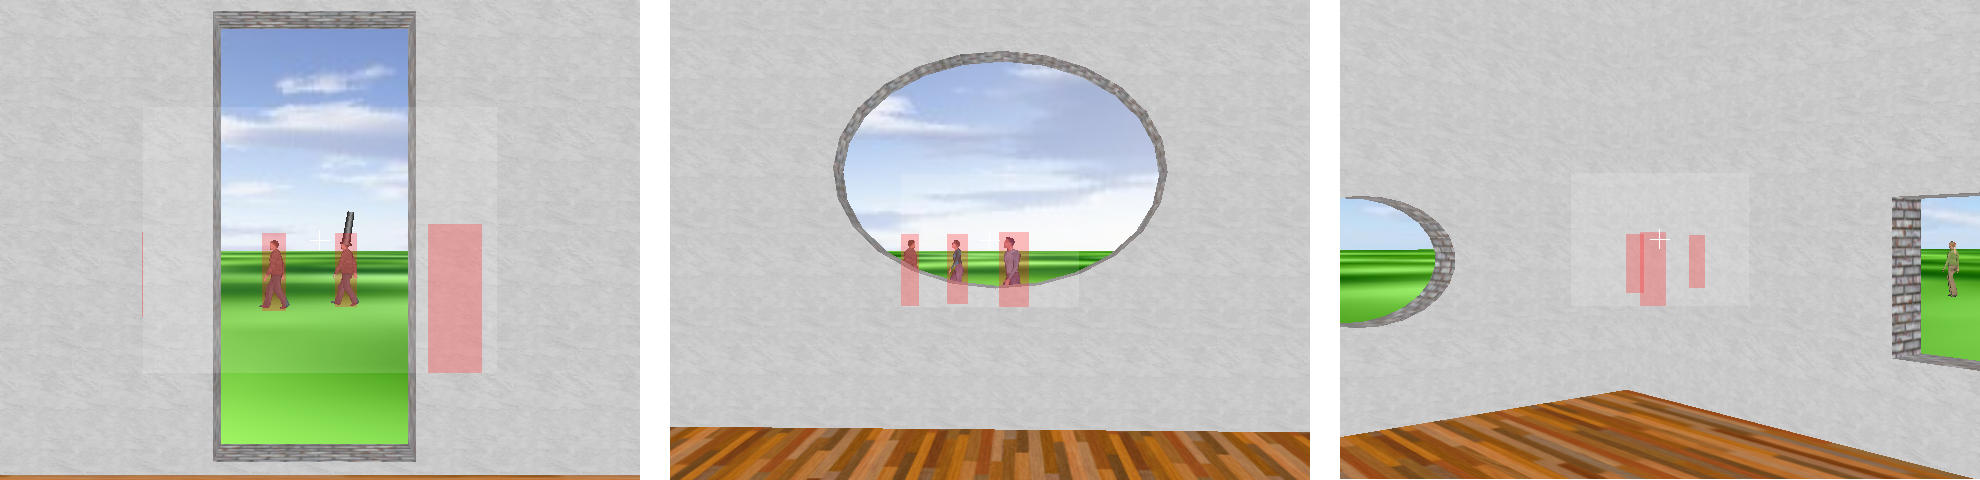
\includegraphics[width=5in]{figures/triple_view.png}
	\caption{Sample views of AR simulation.  Transparent red rectangles overlay the people, indicating their location.  \emph{Left:} A user view of Top Hat (non-occluded) in the doorway.   \emph{Middle:} Three distractor people are visible through a large window.  \emph{Right:} A typical user view of a corner occluding several people.}
\end{figure*}

Our experiment involves a target following task which uses an augmented reality interface to allow people to be tracked behind walls.  A participant stands in the middle of a square room with doors and windows on all sides.  Virtual people walk unpredictable paths outside the building.  The target to be followed is one of these people, visually distinguishable by a large black top hat.  The augmented reality interface overlays a translucent red rectangle on each person, which is visible even when the person is occluded by a wall.  However, the target person's overlay is identical to the other virtual people overlays; the target may only be distinguished when visible through a window or a door.

To actually run this experiment using a true augmented reality system would be extremely difficult.  Many confederates would be needed to walk around the room, and their movements would need to be accurately reproduced for each new participant.  Also, the confederates would need to be continously tracked for the augmented overlays to be displayed.%  Instead, we chose to simulate the experiment setup in a completely virtual environment.%

By simulating augmented reality, we are freed from the current restrictions of display technology.  This simulated environment also affords easily controlled variables, and thus the experiment may be replicated.

\section{Experimental Design}

The design of the experiment is built with several goals in mind.  The task should have straightforward, quantitative results.  Also, the task should be reasonably simple so as not to frustrate the participants.  Further, the task should be generic so as to be generizable, yet grounded in reality (i.e. not an abstract world), to enhance participant familiarity with the AR task.

We developed a target following task scenario, where the user is asked to visually track a virtual person as it moves throughout the scene.  The participant is centered inside a room with various doors and windows giving a view to the outside world.  They may change their orientation, but not change position (3 degrees of freedom).  The user's view to the virtual people may be occluded at any time by the walls of the building; at other times the person may be visible through doors or windows in the building.  The augmented view element is composed of red marker rectangles indicating the location of the person to be followed and distractor people.

The parameters of our experiment are divided between the ``real'' components of immersion, such as the field of view of the HMD, and the ``augmented'' components of immersion, such as the field of view of the simulated AR display, and the performance of the tracking sensor.  We introduce periods of sensor dropouts, where the augmented overlays disappear, to simulate the effect of dropouts in a real tracking system.  For example, such dropouts might occur with a magnetic sensor near interfering material.  Different display options are available in this case; for example we could use the last known sensor reading, or predict future values.
%However, these options could have a positive or negative effect on performance, depending on the circumstances.
However, we determined that hiding the AR overlay during sensor dropouts would have the least effect on performance.

In our experiment we have two independent variables: the field of view of the AR interface and the length of sensor dropout periods.  Each trial is 60 seconds, with seven sensor dropouts.  The total vertical field of view of the HMD is 36 degrees; the three possible values for the augmented field of view were 10, 20, and 34 degrees.  The length of dropouts varied between two seconds (highest), one second (medium) and zero seconds (lowest).  We experimented with longer dropout periods but deemed them too long.  This gave us a total of 9 conditions, and for each participant we tested each condition 3 times giving a total of 27 trials per participant.

During each trial there are 20 people in addition to a virtual man \emph{Top Hat} wearing a tall black top hat walking an unpredictable path outside of the room.  The paths for each virtual person was randomly generated from set of coordinates exterior to the room.  Each path had the constraint that they must stay within the rectangular $50\times50$ $m^2$ area surrounding the room.  At each path point, the person will randomly change his/her walking speed within the range of 4 to 7 m/s.  Top Hat had the additional constraints as follows.  He must start at the same location for each trial which made him visible by the participant through the front door the building.  In order to make the paths by of similar difficulty Top Hat must walk around the entire building at least once, and he must be visible through the windows for at least 10 seconds.  These constraints were met by randomly generating paths until all were satisfied.  We generated 27 sets of paths in this fashion, each corresponding to a specific trial.  We used a latin squares ordering to discourage the effects of learning.

\begin{figure}[t]
	\centering
	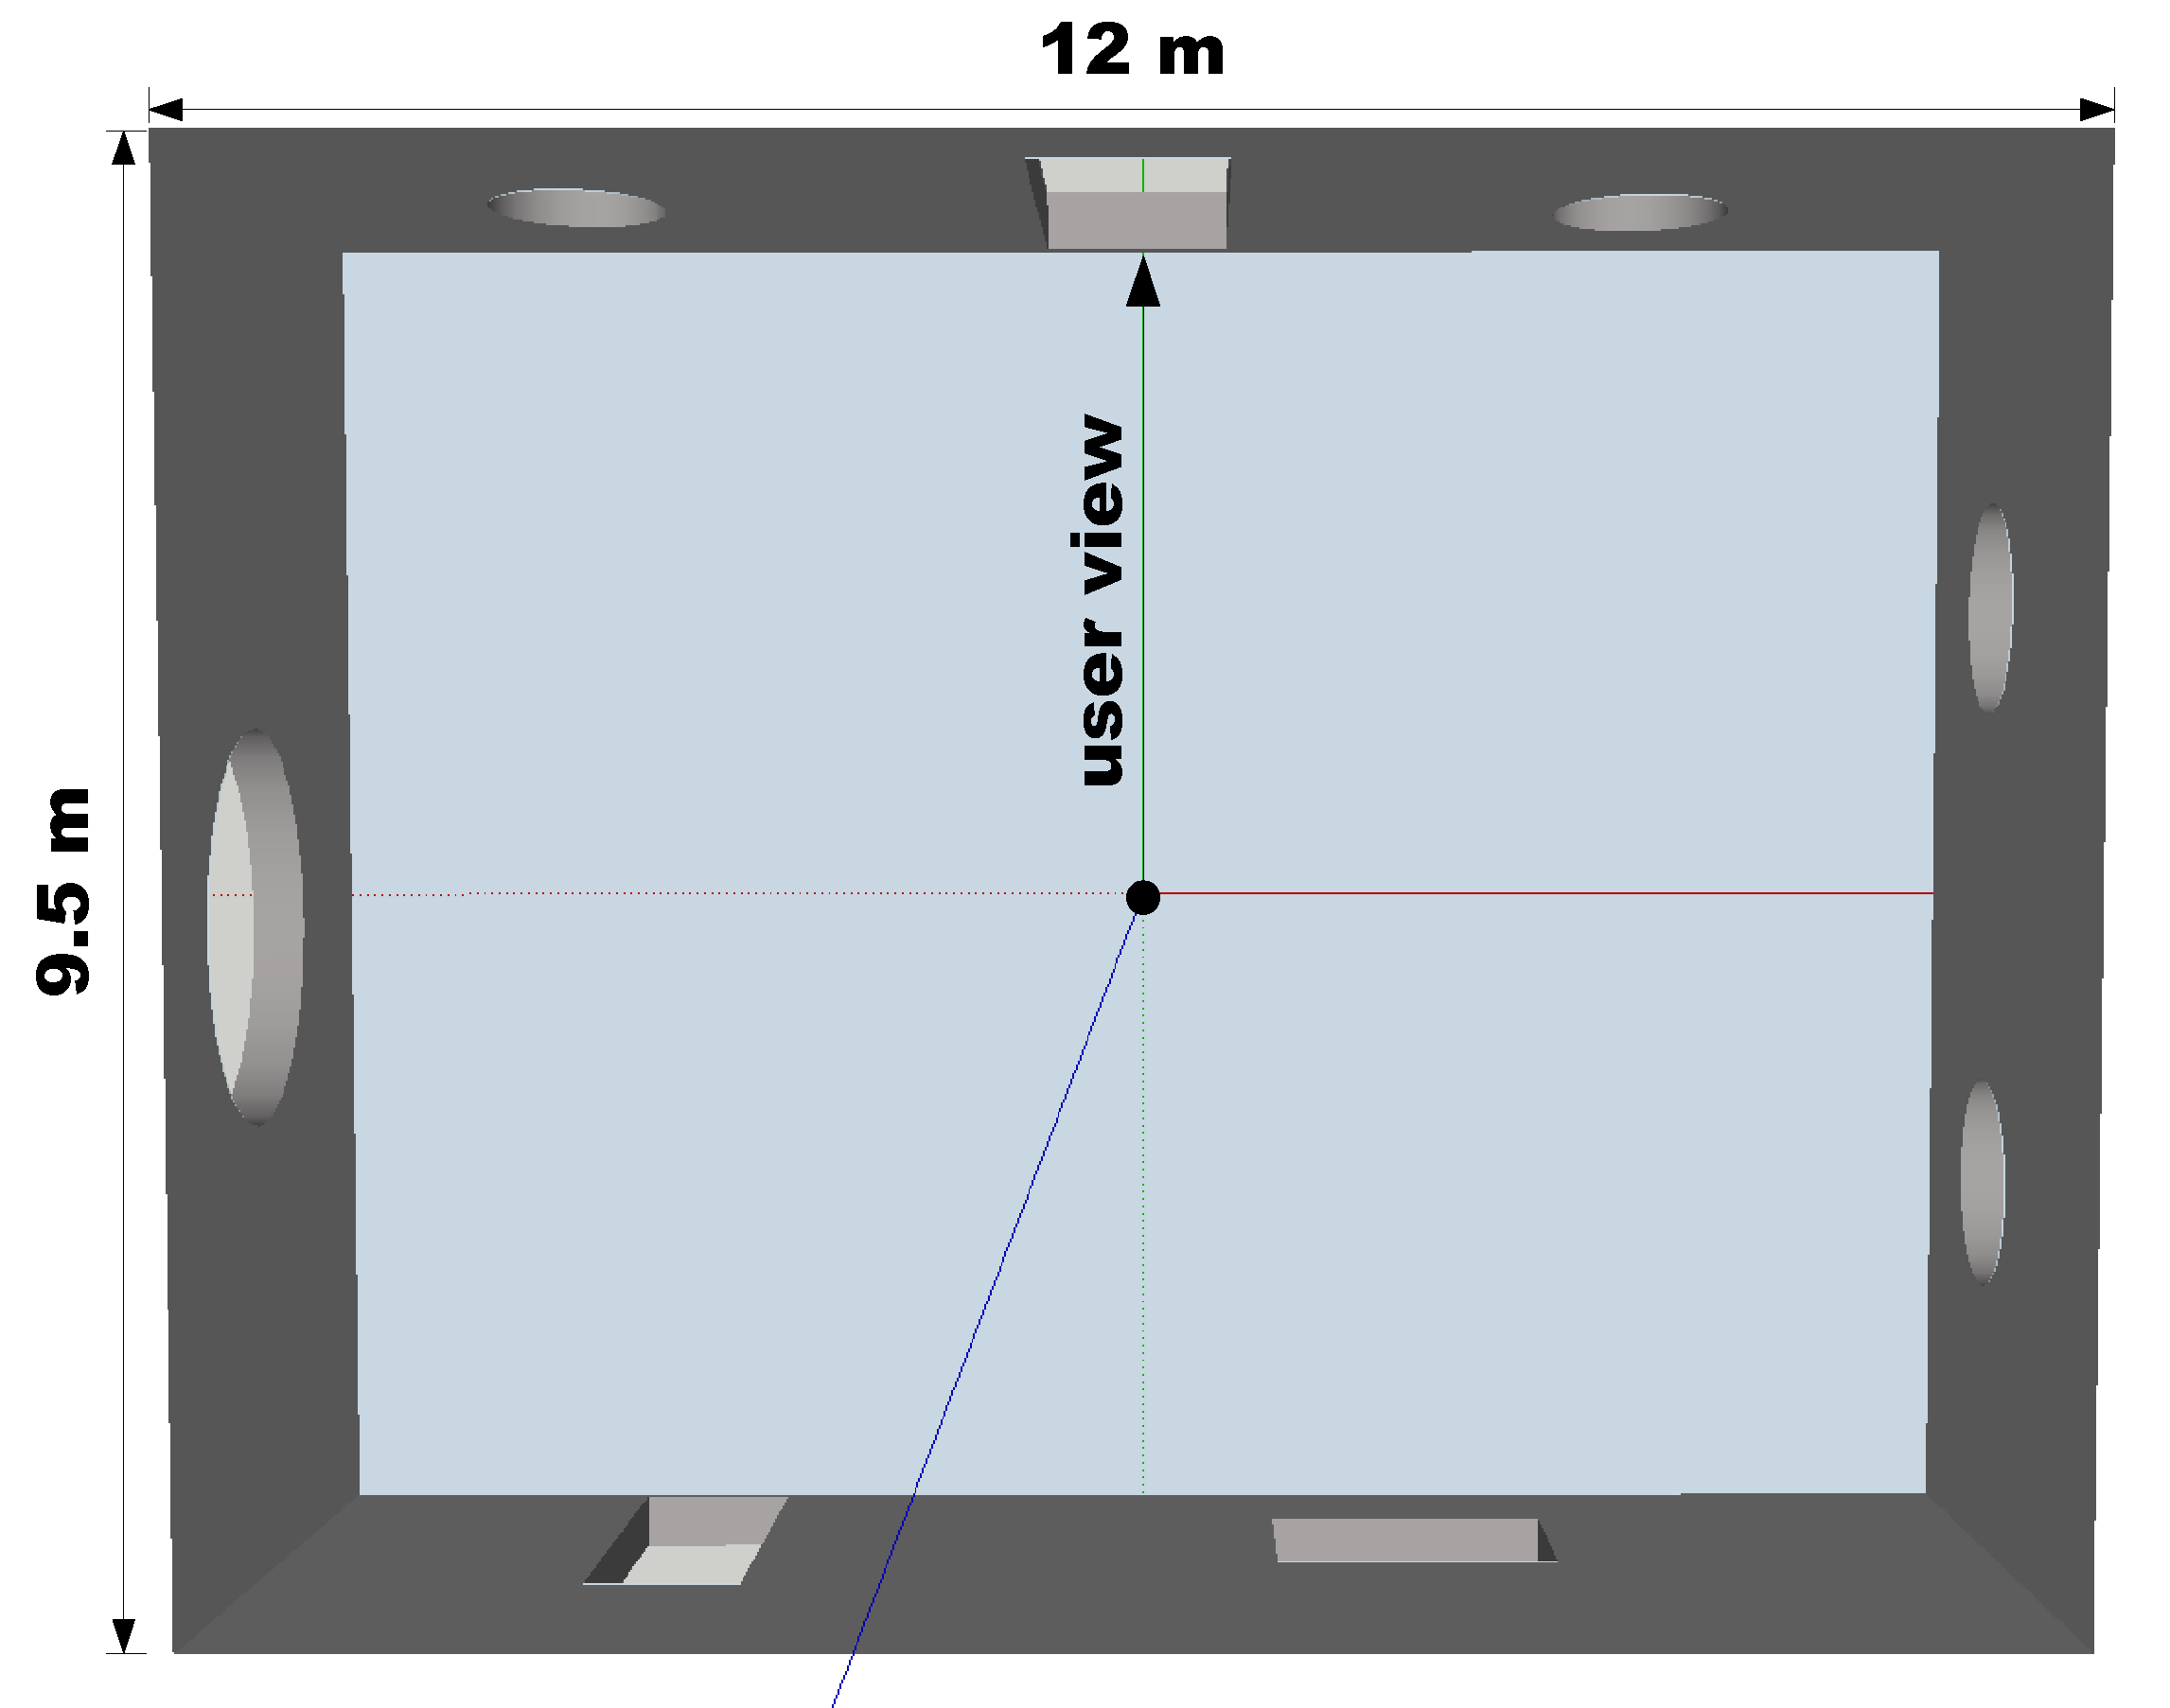
\includegraphics[width=2.5in]{figures/augmentedroom.png}
	\caption{Overhead view of virtual room (approx. measure).  Participant is stationary in the center of the room, with initial orientation along ``user view'' arrow.  Top-hat's initial position is outside the front doorway, directly in the participant's view.}
\end{figure}

\subsection{Implementation}

We implemented this experiment with Python and the Vizard virtual reality toolkit.  Head-tracking was handled by a InterSense InertiaCube3 orientation tracker with a 180 Hz refresh rate.  We used a Pro-View 60 head mounted display (HMD) displaying $640\times480$ video at 60 Hz, and 36 degrees vertical field of view.  As we were not concerned the effects of stereo, we turned off the stereoscopic feature.  The experiment ran on a 2.4 GHz Intel Core 2 machine with 2 Gb of RAM and a NVIDIA GeForce 9800 GX2 graphics card running Windows XP SP3.

\subsection{Participants}

We ran this experiment on 19 subjects, 11 were male, and 8 female.  The participants ranged in age from 23 to 59, 15 were in the range 23 to 30, and the remaining 4 in the range 51 to 49.  None were colorblind.  Most users were heavy computer users with at least somewhat familiarity with virtual reality and augmented reality.  Only one participant played 3D video games often.  After every 9 trials we had the participants take a mandatory 5 minute break.  Some experienced light fatigue, but none experienced any strong effects of motion sickness.

\section{Analysis}

In our experiment we define performance as effectiveness in following Top Hat.  The dependent variable we measure is the angular distance (in yaw) between the the user's viewing direction and the direction towards the target character.  This measure ranges between zero and 180 degrees (we used the smaller of the two options, clockwise and counter-clockwise).  We record one measurement per video frame, at about sixty frames per second, resulting in approximately 3600 measurements for a one minute trial.

Because the video does not always run at precisely 60 Hz, each trial might have a slightly different number of measurements.  We also record a timestamp for each measurement, so that we can determine their exact frequency.  As a pre-processing step, we linearly re-sample the data for each trial so that each has exactly 3600 measurements at 60 Hz.

We observed that participants tend to switch between two different states during the experiment: a target following state, and a lost state, where they are searching for the target.  The two states are easily visible in the data.  In the target following state, the angular error is generally low.  We asked participants to keep the cross hairs on the target as closely as they could, but different participants achieved different levels of accuracy.  In the lost state, the error starts to steadily climb, and may fluctuate depending on where the target moves.  The error may even return to near-zero during a lost state, if the participant unwittingly crosses the target's path.

% TODO: include two plots of error here (one with losses, one without)

%We hypothesize that less immersive conditions will have longer and more frequent periods where the participant loses the target.  We considered several different metrics which might be appropriate in testing this hypothesis.%

The simplest is the average error over an entire trial.  This may not accurately represent sensor dropouts, because the error does not necessarily stay high during the lost state, and also different participants may generally keep the cross hair further from the target even in the target following state.

% median ??

We can more explicitly detect the participant's state by applying a threshold $\tau$ to the data.  The threshold specifies the maximum angular error that still represents successful following of the target. 
%When the error rises above the threshold, we consider the participant lost.
While conducting the trials we noticed that the participants spent a majority of the time correctly following Top Hat, computing the median angular error at each time-step across all trials gave us values mostly around 4 degrees so we consider values close to this as successful tracking.  We also noticed that during trials as Top Hat would change direction the participant's angular error would increase a small amount for a short time, without losing the target.  As a result we doubled the 4 degrees, giving us a threshold of $\tau = 8$ degrees
% TODO: how to motivate this threshold?
\begin{figure}[t]
	\centering
	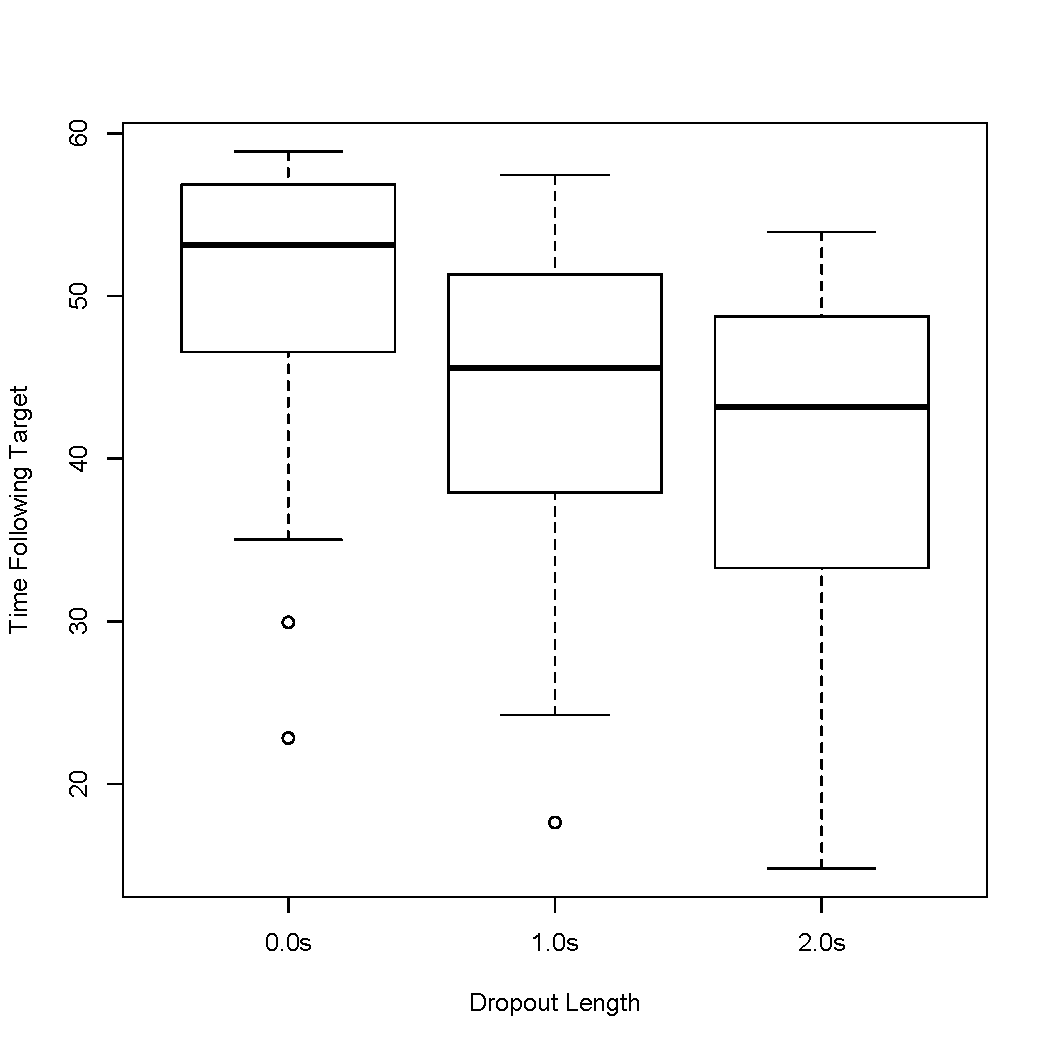
\includegraphics[width=1.5in]{figures/tt_deadlen.pdf}
	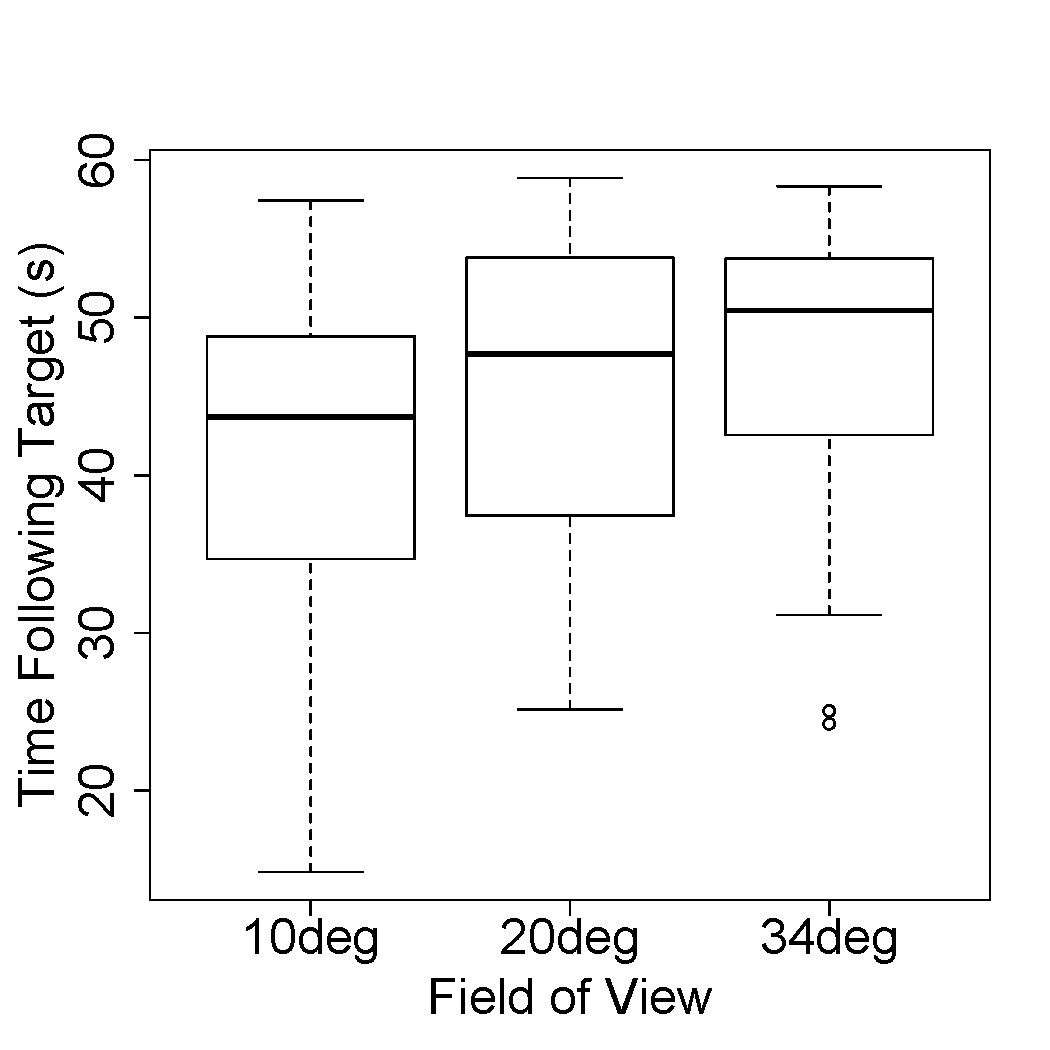
\includegraphics[width=1.5in]{figures/tt_fov.pdf}\\
	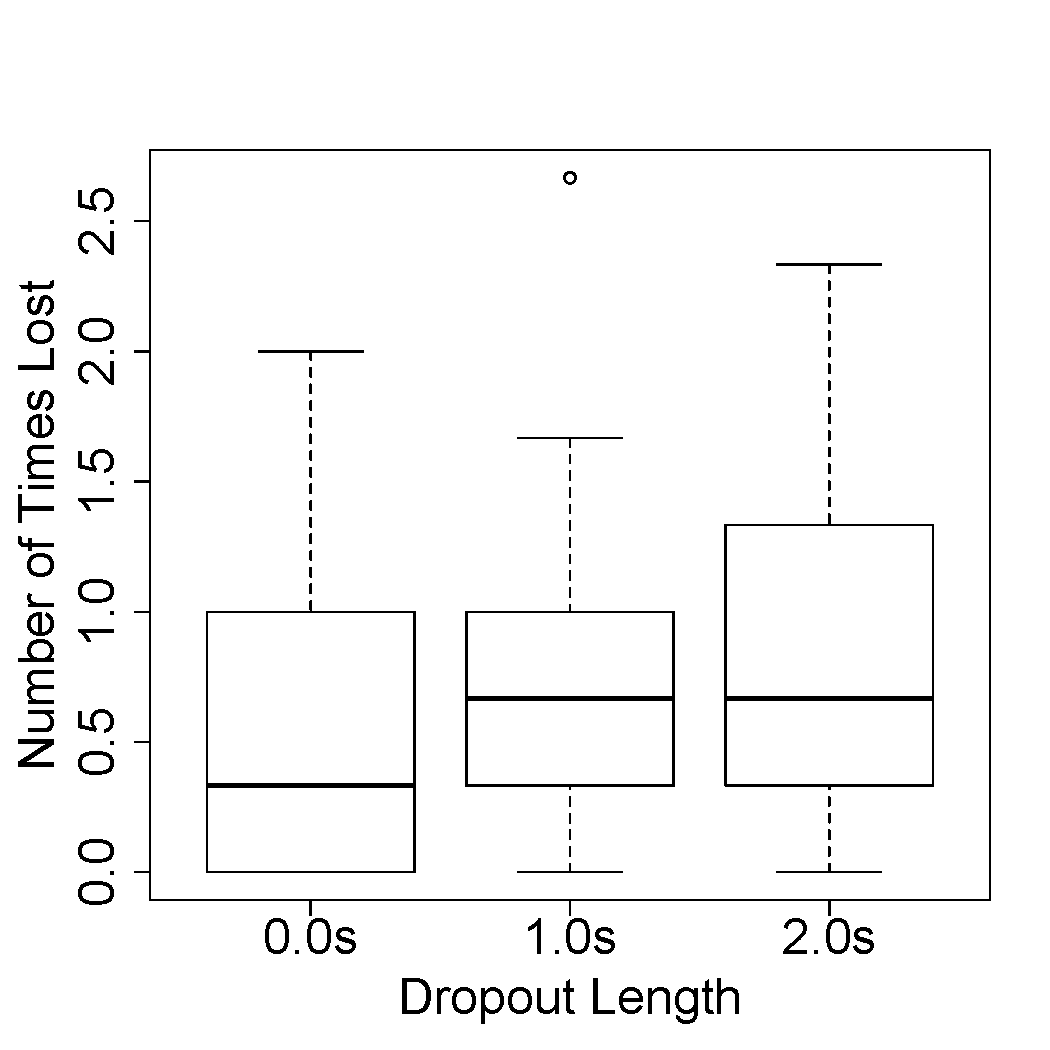
\includegraphics[width=1.5in]{figures/numtimes_deadlen.pdf}
	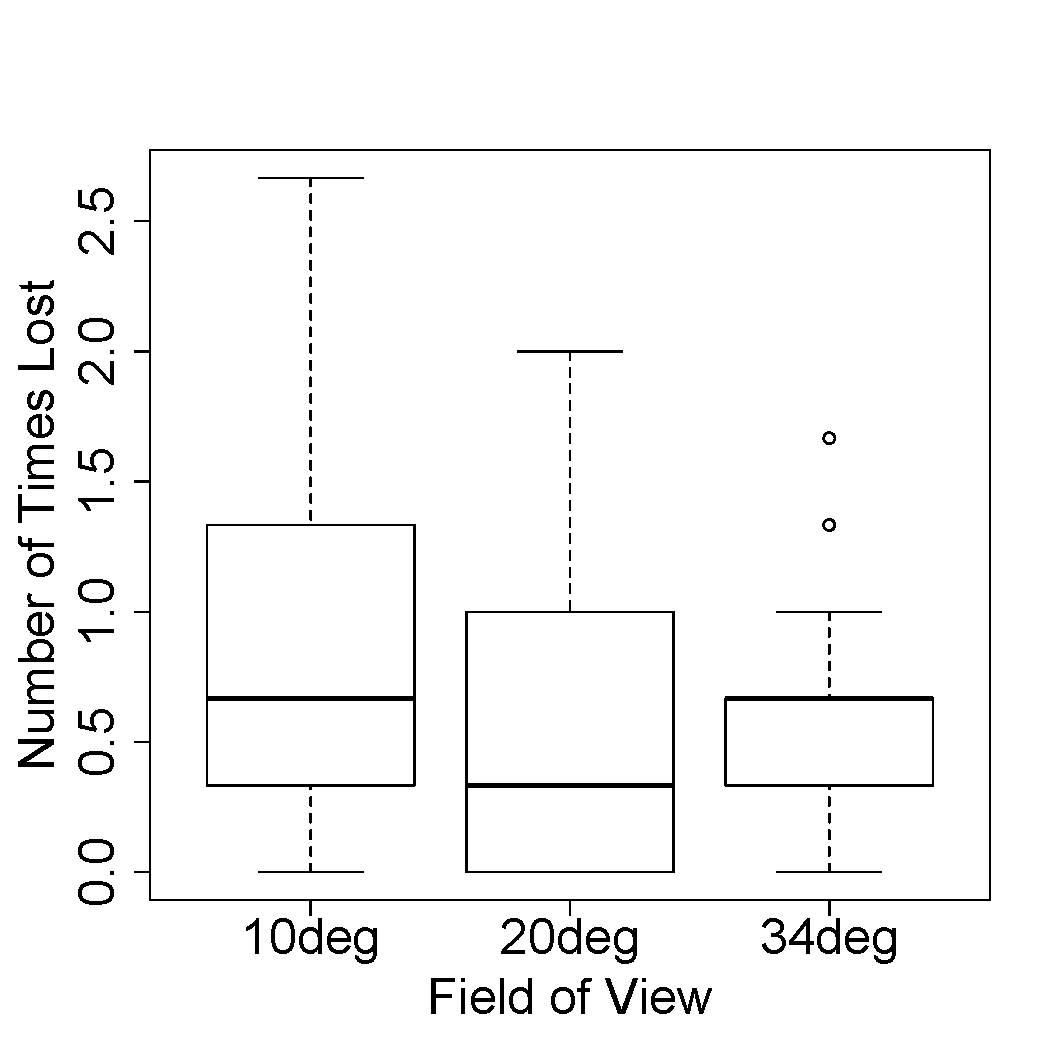
\includegraphics[width=1.5in]{figures/numtimes_fov.pdf}
	\caption{\label{fig:tt_deadlen}Box plots for our two independent variables and two metrics.  In general, performance increases when the length of sensor dropout periods is lessened, and when the AR field of view increases.}
\end{figure}
Using this threshold we measure a participant's \emph{time to failure}, the time until the a lost state is encountered.  However, this may not be a very descriptive measure, since a participant may reach the lost state sooner or later depending on the movement of the avatars, which varies between trials.

We also consider a measurement we call \emph{time following target}, which is the amount of time spent successfully following the target.  This metric seems to most generally represent how well a participant performed.  Trials with either more or longer lost periods will result in a lower total time following the target.

For a more specific measure of performance, we count the number of times a participant reaches the lost state in a trial, or  \emph{number of times lost}.  We only record a lost state when the error stays above the threshold $\tau$ for a minimum of 4 seconds.  A 4 second threshold was used because it is double the maximum dropout length, allowing the user a few seconds to resume successful tracking after the dropout before they are considered to have lost the target.
% TODO: how to motivate this threshold?

%time tracking is overview metric -- captures both number of times lost and length of lost periods

%number of times lost is piece of overview -- number of times lost.

\section{Results}

%\begin{figure}[t]
%	\centering
%	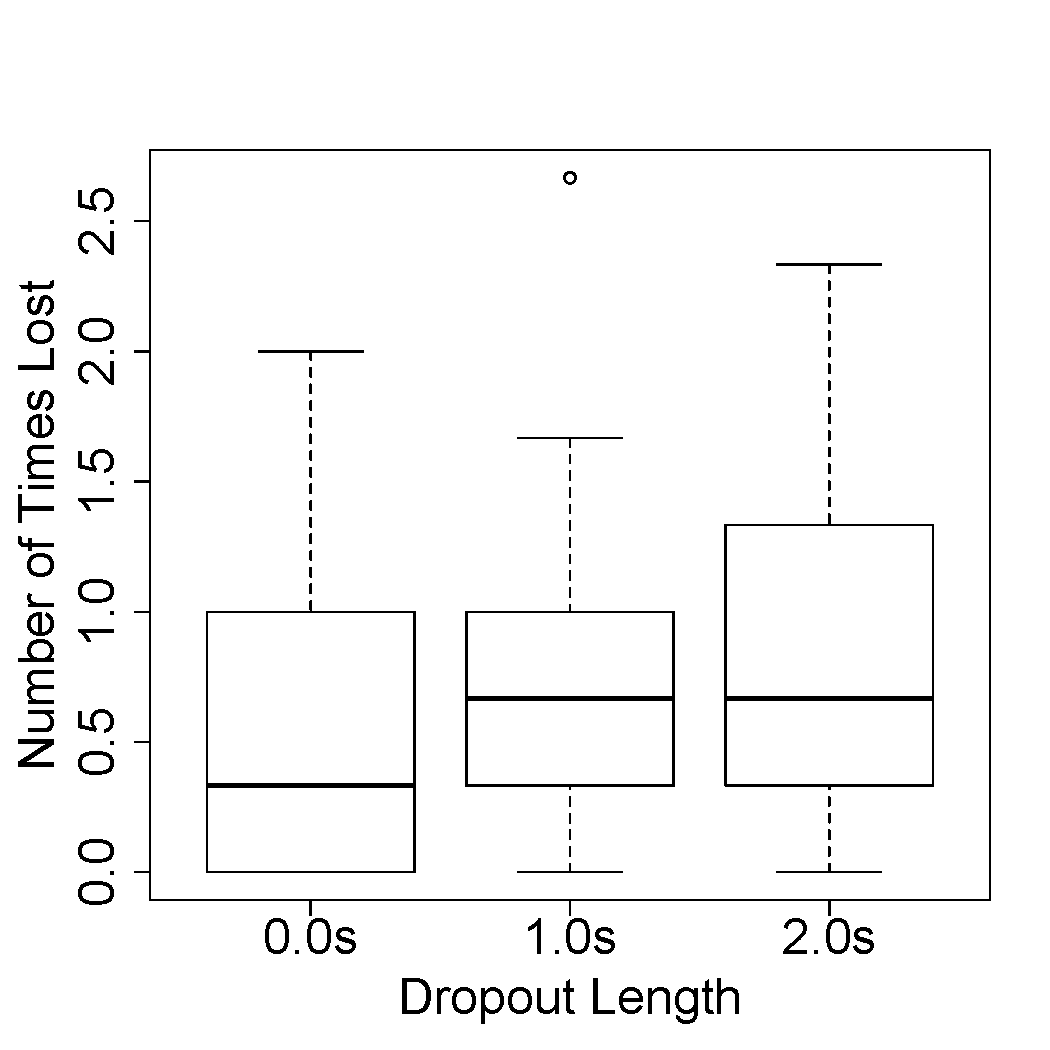
\includegraphics[width=3in]{figures/numtimes_deadlen.pdf}
%	\caption{Box plot of the number of times the participant is lost versus the length of the sensor dropouts.}
%\end{figure}

%\begin{figure}[t]
%	\centering
%	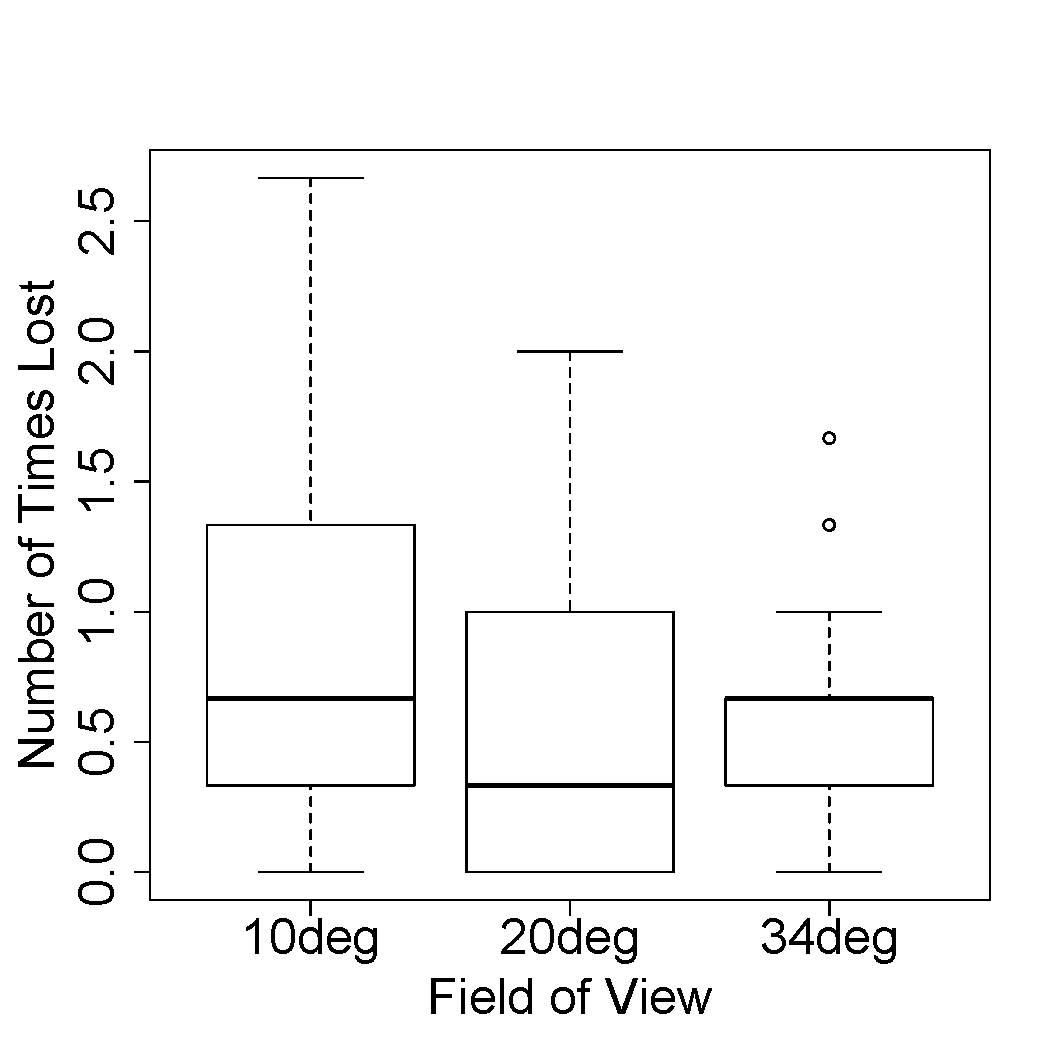
\includegraphics[width=3in]{figures/numtimes_fov.pdf}
%	\caption{Box plot of the number of times the participant becomes lost versus the field of view of the augmentations.}
%\end{figure}

% TODO: make the units seconds and change the labels on the bottom of this figure


%\begin{figure}[t]
%	\centering
%	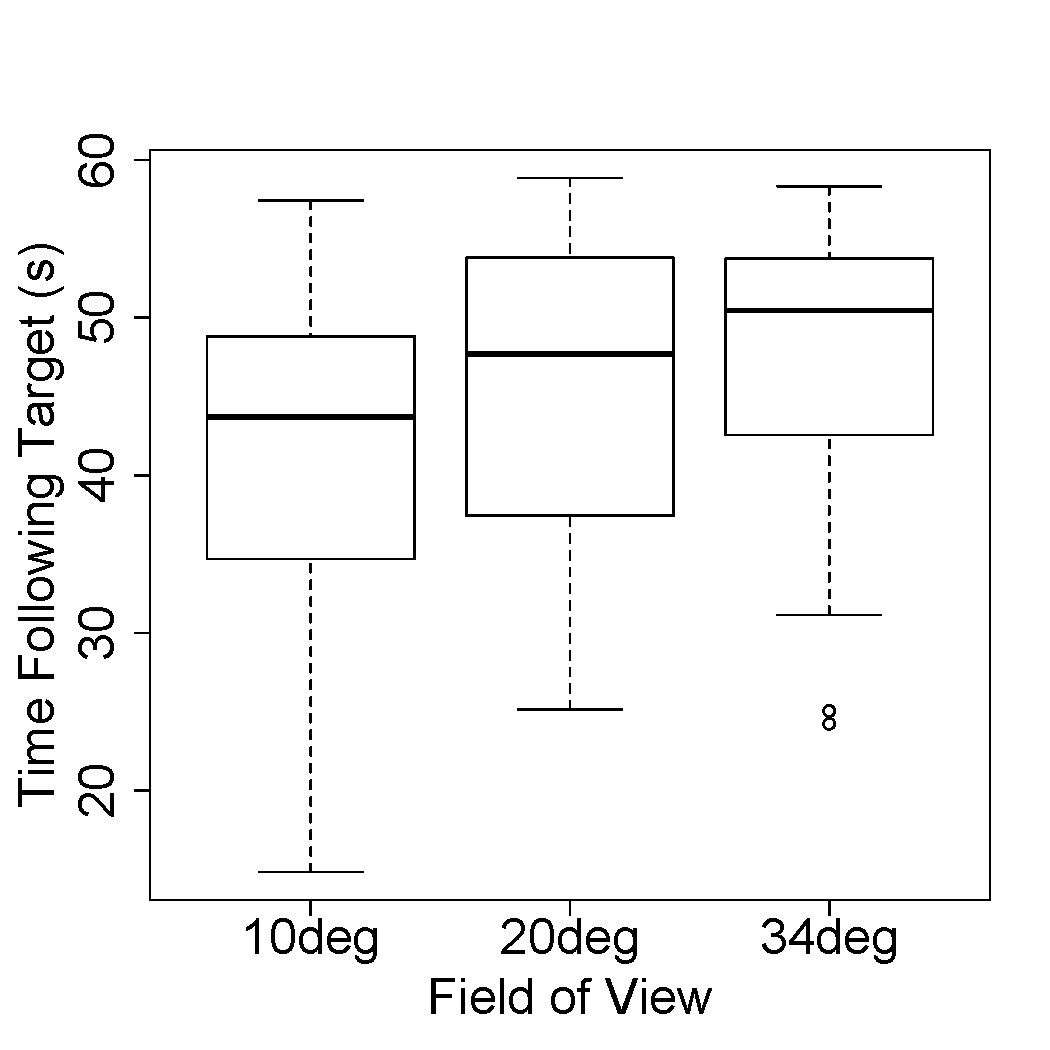
\includegraphics[width=3in]{figures/tt_fov.pdf}
%	\caption{Box plot of time the participant is not lost versus the field of view of the augmentations.}
%\end{figure}


% TODO: should we include data from older generation??

% TODO: look at analysis from mean.

We performed two-way {ANOVA} for the time following target metric as an overall analysis of the effects of our two factors.  Figure \ref{fig:anova} gives the results of this analysis.  Both the failure length and the field of view have a very significant effect on performance using this metric.  
% TODO: interaction?

We also used a two-way {ANOVA} to examine the number of times the participant loses the target, with results shown in Figure \ref{fig:anova}.  Both field of view and dropout length have a significant effect.  There also is an interaction between the two factors.  Figure \ref{fig:interaction} shows a plot of this interaction.  
% TODO: need F values reported here.

From this plot we can see that with a small field of view, performance is equally bad with no dropouts or one second dropouts.  
%The small field of view seems to have a dominating effect on performance.  
When the field of view is increased to the medium level, performance dramatically increases when there are no dropouts, but only gets slightly better when there are dropouts.  Finally, there is not a significant difference in performance between the medium and large field of view ($p=0.575$), which suggests that the medium field of view is enough for good performance.
%Finally, we do not observe much difference in performance between the medium and large field of view cases.  Using Tukey's HSD to compare means, the medium and large field of view conditions are in fact not significantly different ($p=0.575$).

\begin{figure}[t]
	\centering
	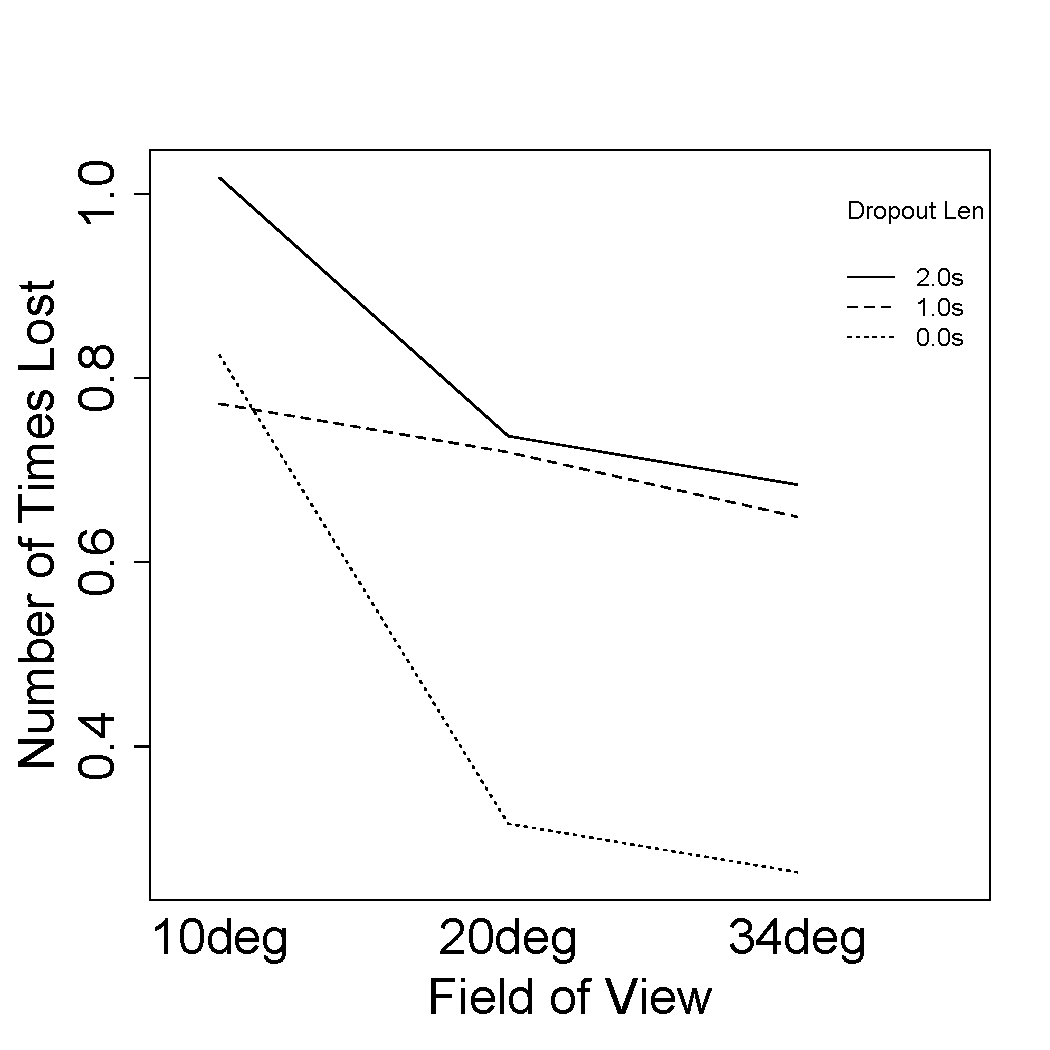
\includegraphics[width=2.5in]{figures/numtimes_interaction.pdf}
	\caption{\label{fig:interaction}Interaction plot of the effect of field of view and sensor dropout length on the number of times the participant loses the target.}
\end{figure}

\begin{figure}[h]
\centering
\begin{tabular}{|c|c|c|c|}
\hline
%\multicolumn{2}{|c|}{Selection Stroke Thresholds} \\
Metric & Factor & F value & Pr \\
\hline
Time Following Target & Dropout Length & 28.904 & $<0.001$\\
Time Following Target & Field of View & 15.800 & $<0.001$\\
Number of Times Lost & Dropout Length & 8.5008 & $<0.001$\\
Number of Times Lost & Field of View & 13.060 & $<0.001$\\
\hline
\end{tabular}
 \caption{\label{fig:anova}Factors which have a significant effect.}
\end{figure}

Figure \ref{fig:tt_deadlen} shows a box plot of time following target versus dropout length.  Performance decreases between zero and one seconds, but seems to level off between one and two.  We ran a post-hoc analysis to determine which conditions were significantly different.  Using Tukey's HSD, we found that the one second and two second conditions were significantly different than zero ($p<0.001$ for both), but not significantly different from each other ($p=0.239$).  This suggests that we may be seeing a thresholding effect above one second sensor dropouts.
% TODO: table with values

To investigate this threshold, we had seven participants complete an extra three trials with the medium field of view and sensor dropout periods of 0.5 seconds.  Figure \ref{fig:extra} shows a box plot of time following target versus sensor dropout length for these seven participants.  Again using Tukey's HSD to compare the means, we did not find a significant difference between the zero length and half second length conditions, but did find a significant difference between those and the higher length conditions.
%TODO: table with values
With further experimentation, we could further delineate the performance curve as the dropout length increases from zero to one.

\begin{figure}[htb]
	\centering
	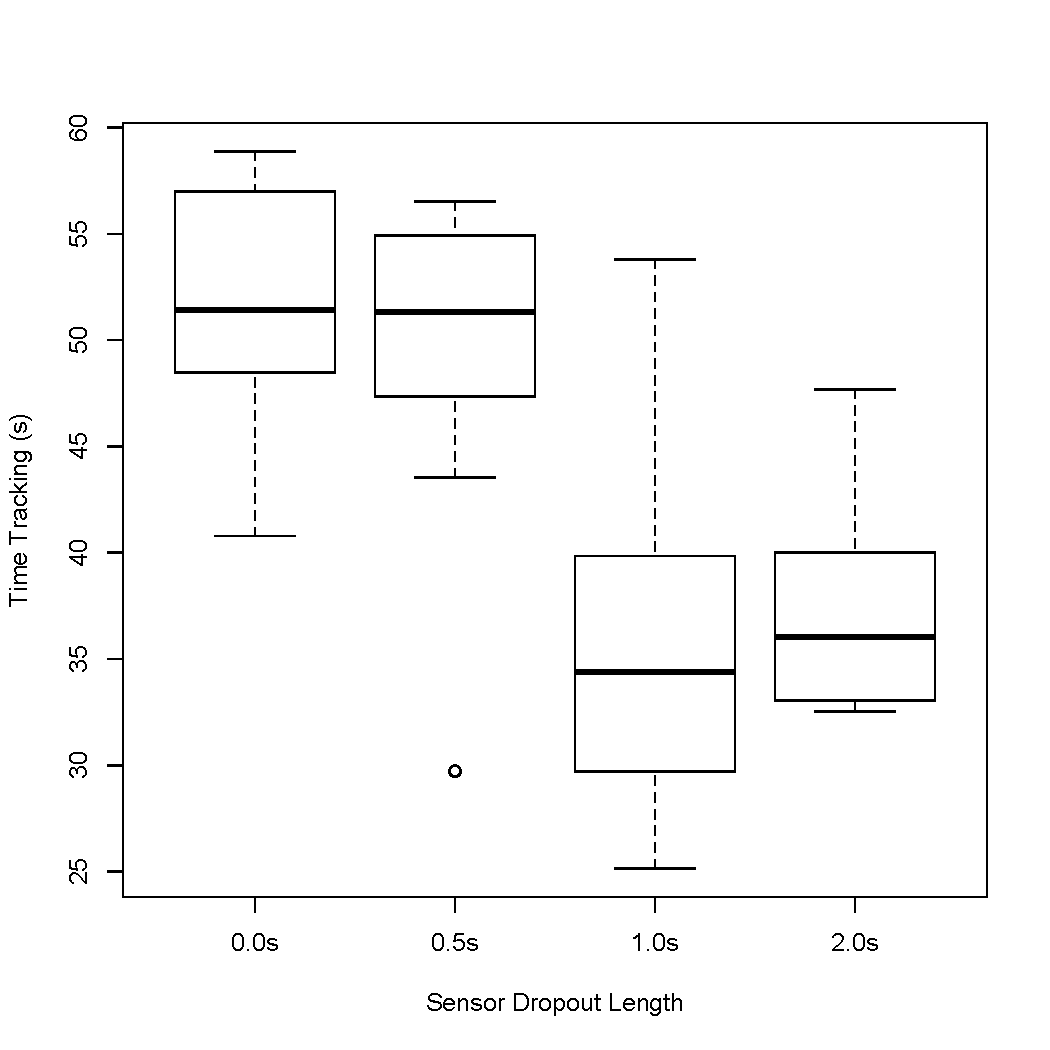
\includegraphics[width=2.5in]{figures/extra.pdf}
	\caption{\label{fig:extra}Box plot of the total time the participant is following the target versus the length of the sensor dropout periods, including the half second dropout condition.  We collected this data from seven participants, using the medium field of view.}
\end{figure}

%use multiple comparison of means to determine which pairs are significant -- difference between length of one and length of two is not significant.

\section{Conclusions and Future Work}

We designed a AR experiment to study the effects of tracker reliability and field of view on a target following task.  We developed a virtual reality based AR simulation to enable control over these independent variables.

We found that for our task, a low field of view has an adverse effect on performance.  
%This adverse effect dominates the other variable component of immersion, the reliability of the head-based rendering.
With reliable head-based rendering, a medium field of view is enough for good performance.  We did not see a significant performance increase when increasing to a high field of view.

Decreased reliability in the head-based rendering, caused by periods of sensor dropout, adversely affects performance.  However, the performance decrease levels off at one second dropouts.  Preliminary analysis also shows no significant difference between having no dropouts and half second dropouts.  This suggests that below a certain length of dropout time, good performance may be maintained, given a sufficiently large FOV.%  This threshold on dropouts would change depending on the task at hand, but we expect the same pattern would arise in other target following scenarios.

Future work lies in further investigating the effect of the dropout length 
below the one second level.  Our work also suggests new experiments designed to test the interaction between reliability of the head-based rendering and various other immersion components.

%\section*{Acknowledgements}
%Cha Lee, Steffen Gauglitz, funding, and all of our participants.

\bibliographystyle{acmsiggraph}
\bibliography{paper}
\end{document}
